\chapter{Implementación} \label{implementacion}
\section{Prueba de concepto} \label{implementacion.prueba}

La primera fase de desarrollo de la solución fue la prueba de concepto; su objetivo fue encontrar las herramientas adecuadas para el \textit{Stack Tecnológico} y demostrar que las elegidas son viables y que funcionan en conjunto. Además, se estudiaron y valoraron los problemas que puedan presentar y los retos que podrían suponer desde una aproximación tecnológica. Conceptualmente, este apartado podría verse englobado dentro de la sección de Análisis (Capítulo \ref{analisis}) ya que, como se ha mencionado, la prueba de concepto fue la que determinó el \textit{Stack Tecnológico} y, por ende, incluyó una correspondiente parte de análisis, esto es, búsqueda, investigación, test de viabilidad, etc. No obstante, dado que realmente formó parte del desarrollo de la solución se ha decidido redactarlo como una primera parte del apartado de Implementación de la solución. Así pues, esta sección presentará tanto el \textit{Stack Tecnológico} utilizado, los problemas encontrados en esta fase y las diferentes alternativas que se han probado junto con los motivos por los que se han desechado de la decisión final. En el diagrama de la figura \ref{fig:pruebaconceptoglobal} se puede observar el panorama global de los pasos que se han dado y las herramientas que se han utilizado para montar toda la infraestructura necesaria para una versión final de la prueba de concepto dentro de la primera fase del desarrollo del proyecto. 
\par Después se hará un breve resúmen de las pruebas que se han realizado con las diferentes herramientas consideradas como partes potenciales del \textit{Stack Tecnológico}, que será ampliado en la sección \ref{e.disenyo.pruebaconcepto} de los Anexos.
\begin{landscape}

\begin{figure}[p!]
    
    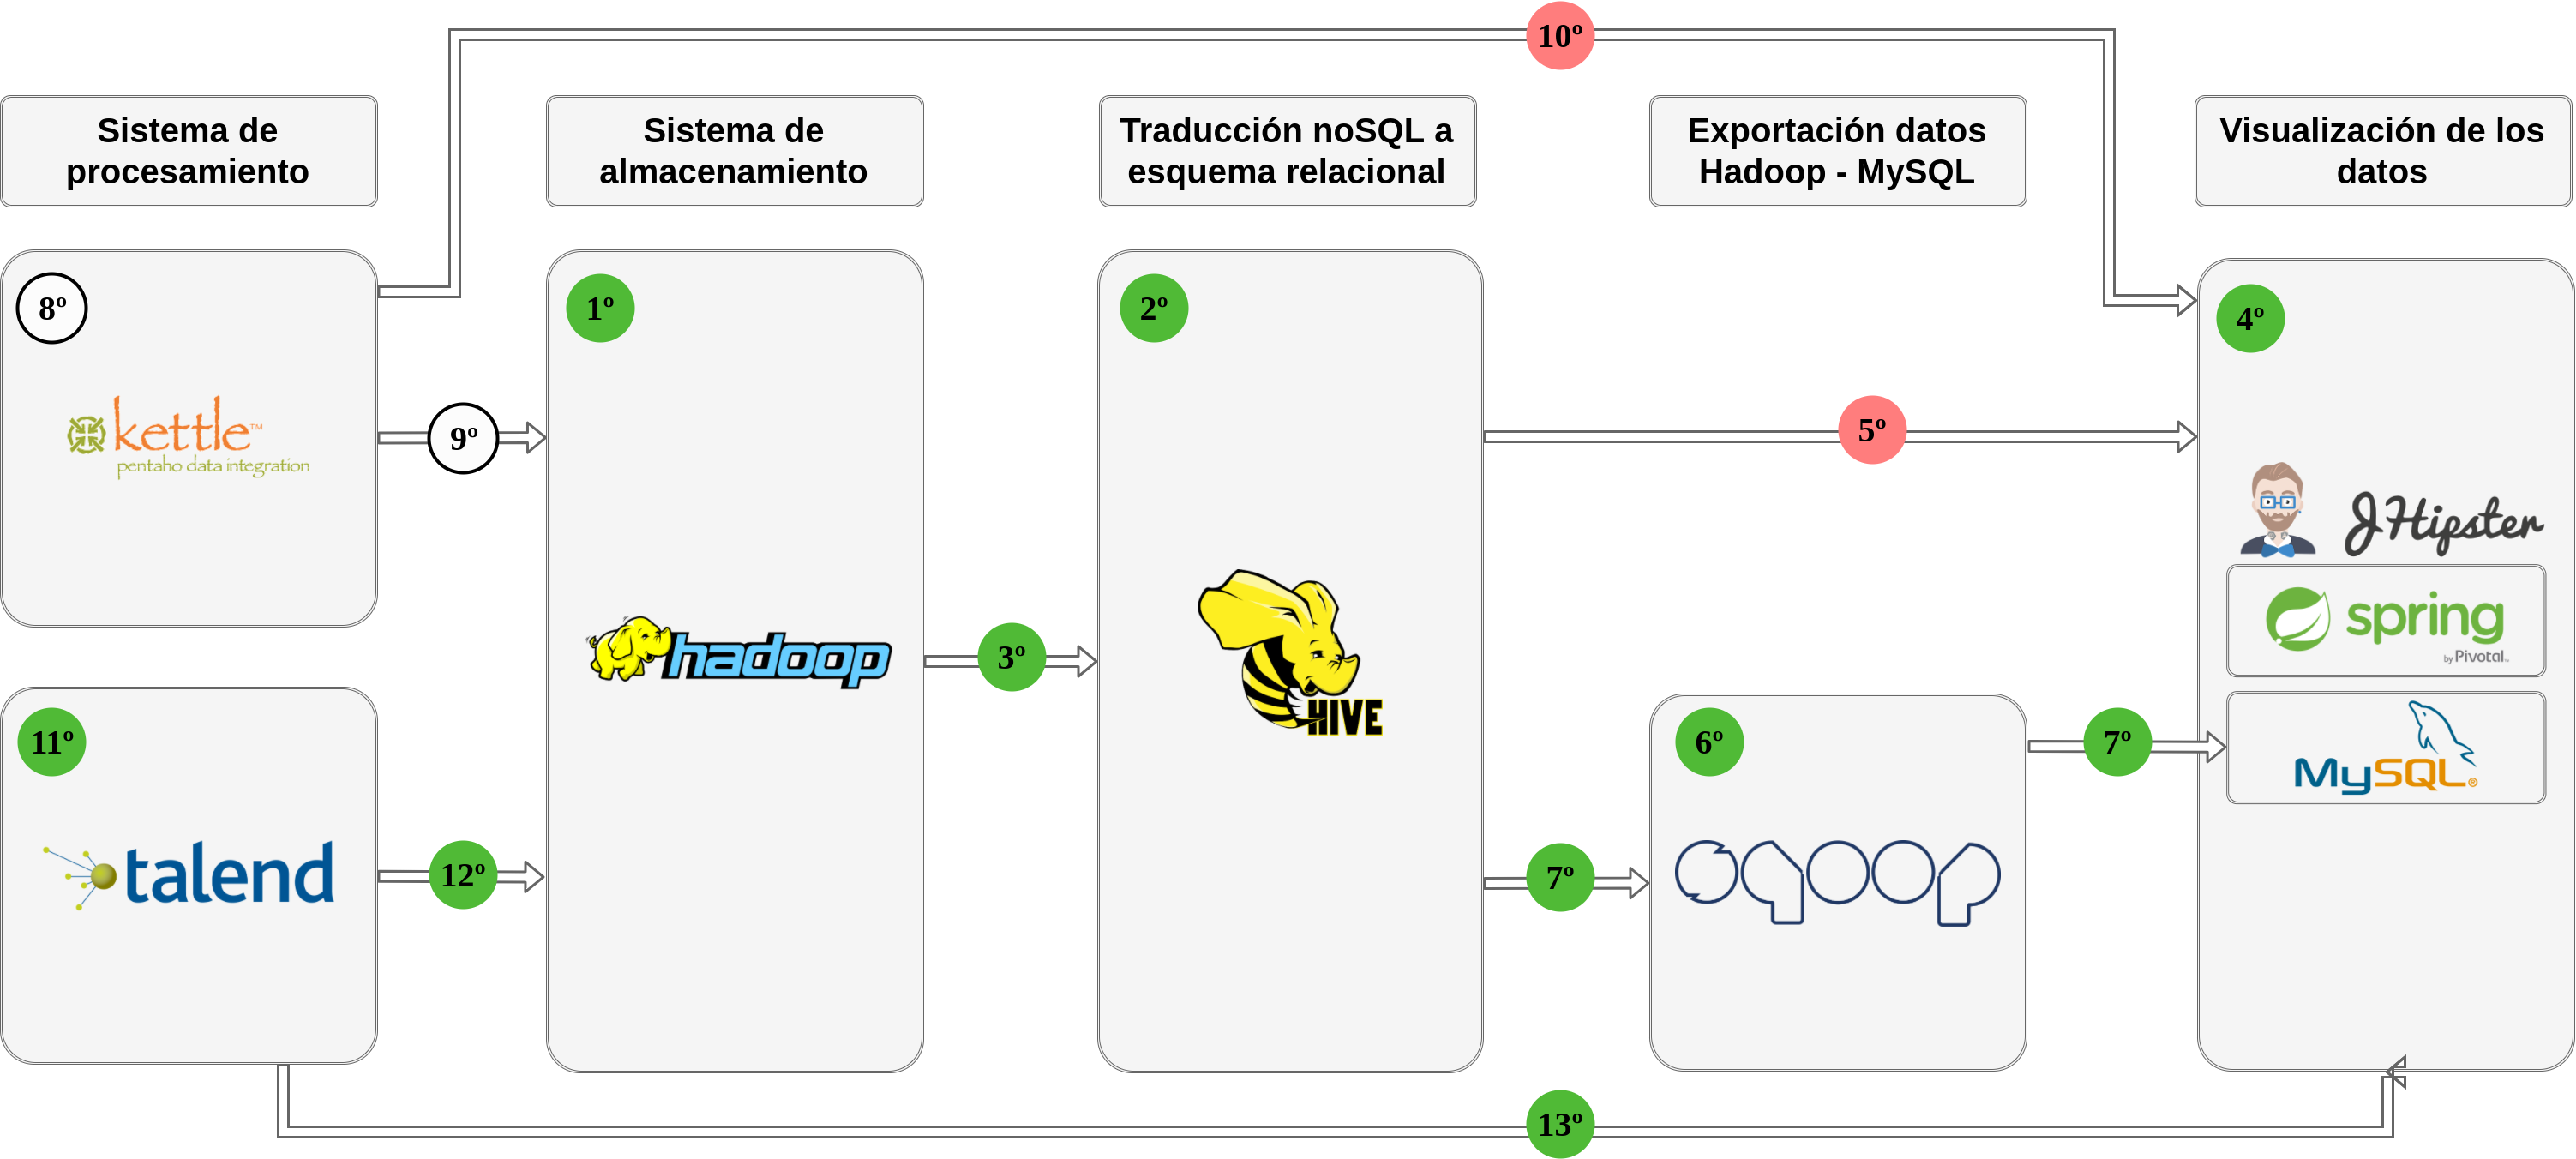
\includegraphics[width=\linewidth]{Imagenes/pruebadeconceptoglobal}
    \caption{Diagrama de las etapas de la prueba de concepto.}
    \label{fig:pruebaconceptoglobal}
\end{figure}

\end{landscape}


\par

\textbf{Pasos reflejados en el diagrama de la figura \ref{fig:pruebaconceptoglobal}:}
\begin{itemize}
\item \textbf{1º.} Instalación y configuración de \textit{Apache Hadoop}.
\item \textbf{2º.} Instalación y configuración de \textit{Apache Hive}.
\item \textbf{3º.} Configuración de la conexión de \textit{Apache Hadoop} con \textit{Apache Hive}.
\item \textbf{4º.} Instalación y configuración de \textit{JHipster}.
\item \textbf{5º Fallido.} Intento fallido de conexión directa entre \textit{JHipster} y \textit{Apache Hive}.
\item \textbf{6º.} Instalación y configuración de \textit{Apache Sqoop}. 
\item \textbf{7º.} Exportación de datos desde \textit{Apache Hive} a \textit{MySQL} (base de datos de \textit{JHipster}) con \textit{Apache Sqoop}.
\item \textbf{8º.} Instalación y configuración de \textit{Kettle Pentaho}.
\item \textbf{9º.} Desarrollo de procesos \textit{ETL} para \textit{Apache Hadoop} mediante \textit{Kettle Pentaho}.
\item \textbf{10º Fallido.} Intento fallido de importación de procesos de \textit{Kettle Pentaho} en \textit{JHipster}.
\item \textbf{11º.} Instalación y configuración de\textit{ Talend Big Data}.
\item \textbf{12º.} Desarrollo de procesos \textit{ETL} para \textit{Apache Hadoop }mediante \textit{Talend Big Data}.
\item \textbf{13º.} Importación de procesos de \textit{Talend Big Data} en \textit{JHipster}.
\end{itemize}


\par
\paragraph*{Desarrollo de la prueba de concepto.}
Tal como se observa tanto en el diagrama como en los pasos anteriores, la prueba de concepto se llevó a cabo de una manera secuencial, validándo primero las tecnologías y herramientas individuales y posteriormente intentando integrárlas. En primer lugar \textit{(pasos 1 y 2)} se instalaron y configuraron los componentes principales del proyecto: \textit{Apache Hadoop} y \textit{Apache Hive} y después se llevó a cabo su interconexión guiada por pruebas de traspaso de datos de \textit{Hadoop} a \textit{Hive} \textit{(paso 3)}. A continuación se instaló \textit{JHipster} \textit{(paso 4)} y en una primera aproximación al problema se intentó conectar diréctamente \textit{JHipster} con la base de datos \textit{Hive} \textit{(paso 5)}. Tras descubrir que este método no era adecuado pues \textit{JHipster} no ofrece ningún tipo de soporte \textit{ad hoc}, se optó por un cambio de estrategia; enlazar el flujo de datos entre \textit{Hive} y \textit{JHipster} mediante \textit{Sqoop}. Para ello se instaló, configuró y probó \textit{Sqoop} \textit{(pasos 6 y 7)} con resultados satisfactorios. Tras observar que el uso exclusivo de estas herramientas eran incompletas para el desarrollo del proyecto (puesto que se determinó necesario un programa de procesado, transformación y carga de ficheros), la opción más prometedora fue \textit{Kettle Pentaho} \textit{(paso 8)}. Si bien la construcción de los procesos mediante esta herramienta resultó una tarea no demasiado tediosa \textit{(paso 9)}, su traspaso a un programa \textit{Java} integrable dentro del proyecto de \textit{JHipster} resultó reiterádamente fallido \textit{(paso 10)}. Se decidió recurrir a otra prometedora herramienta, \textit{Talend Big Data} como sustitutiva de \textit{Kettle Pentaho}, lo que resultó en una gestión acertada \textit{(paso 11)}. 
Con \textit{Talend} se pudieron construir los procesos necesarios para transformar y transportar los datos desde/hacia \textit{Hadoop} \textit{(paso 12)} y se logró realizar el traspaso de dichos procesos a un programa \textit{Java} e integrarlo en \textit{JHipster} \textit{(paso 13)}.

\par
\paragraph*{Conclusiones.}

\par
Una vez conseguidos los pilares fundamentales de la integración dentro del proyecto (\textit{Hadoop}, \textit{Hive}, \textit{JHipster}, \textit{Sqoop}, \textit{Talend}) realmente las únicas preocupaciones que quedaban eran la automatización íntegra del proceso y la ejecución periódica del mismo para disponer de los datos en su versión actualizada. No obstante, para estas tareas no fue necesaria una prueba de concepto puesto que todo esto se podía conseguir desde el propio proyecto de \textit{JHipster}, mediante \textit{Spring} y código \textit{Java}, cosas con las que el alumno ya estaba familiarizado. Dándo por finalizada la prueba de concepto, se empezó a diseñar y construir el prototipo real que quedaría como solución real del proyecto.


\section{Prototipo} \label{implementacion.prototipo}
\par 
\textbf{Primera iteración para conseguir una integración y automatización completa - Productos fitosanitarios autorizados de España}
\bigskip
\par Lo primero que se hizo entrando en el desarrollo del prototipo real fue implementar un simple proceso mediante la interfaz gráfica de \textit{Talend}. Este proceso realiza las siguientes operaciones: 
\begin{enumerate}
\item Descarga desde la web del \textit{Mapama} el fichero \textit{Excell} de los productos fitosanitarios autorizados.
\item Convierte dicho \textit{Excell} a un formato \textit{OpenOffice} para poder ser procesado desde \textit{Talend} con los componentes excel correspondientes. 
\item Sube a Hadoop una versión sin procesar del fichero
\item Procesa el fichero añadiendole una columna llamada \textit{ID} al principio y lo sube como versión procesada a \textit{Hadoop}. 
\end{enumerate} 

A continuación se exportó el proceso desde Talend: 
\textit{Archivo $\rightarrow$ Export $\rightarrow$ Java $\rightarrow$ JAR file}. Esto exporta las clases y librerias que \textit{Talend} necesita para lanzar el job en un archivo comprimido llamado \textit{nombre\_job.jar}
El siguiente paso fue descomprimir el \textit{JAR} en cuestión, analizar su contenido y ver cómo se podría importar en un proyecto Java. El \textit{JAR} contenía varias carpetas y ficheros pero lo que interesa es lo siguiente:
\bigskip
\par 
\dirtree{%
.1 Nombre\_del\_jar.
.2 lib.
.3 \textit{librerias jar}.
.2 Nombre\_del\_proyecto.
.3 Nombre\_del\_job.
.4 \textit{clase java principal del job}.
.2 routines.
.3 system.
.4 api.
.5 \textit{clases java}.
.4 xml.
.5 sax.
.6 \textit{clases java}.
.4 \textit{clases java}.
.3 \textit{clases java}.
}
\bigskip
\par
Así pues, a continuación se creó un nuevo proyecto \textit{Java} con \textit{IntelliJ} y \textit{Maven} (\textit{TalendCrawler}) y se copiaron todas las clases Java con su correspondiente estructura de carpetas. Dentro del fichero pom.xml del proyecto \textit{TalendCrawler} donde se importaron todas las dependencias de Talend que figuraban como librerías locales en la carpeta \textit{lib}. Para ello se tuvo que definir el \textit{repositorio de paquetes de Cloudera} \cite{cloudera}, que es desde donde Maven buscaría la mayoría de librerías. Tras comprobar que la aplicación arrancaba y se comportaba correctamente, el próximo paso fue encapsular y exportar la aplicación como un \textit{JAR}, en conjunto con sus librerías. Para ello se hizo uso del plugin \textit{one-jar} de \textit{Maven} que recoge las dependencias del proyecto y las empaqueta junto a las otras clases en un único \textit{JAR}.\par 

En el proyecto de \textit{JHipster} lo que se hizo fue crear una clase llamada Talend, desde la que periódicamente (mediante \textit{@Scheduled}) se ejecutaba el \textit{JAR} anterior a través del comando \textit{Runnable}. 

\par
Teniendo ya el proceso de \textit{Talend} integrado en la aplicación de \textit{JHipster}, el siguiente problema a abordar fue el de la automatización de su ejecución. Se sabe que los productos fitosanitarios autorizados son actualizados periódicamente en la web de \textit{Mapama}. Por eso mismo, nuestra aplicación requería también de una descarga periódica de dichos datos, para asegurarse de que en todo momento el programa tiene la versión actualizada de los fitosanitarios autorizados de España. Esto se consiguió gracias al \textit{módulo de scheduling}\cite{spring_scheduling} de \textit{Spring} que permite programar la ejecución de un método de manera periódica. Como decisión estratégica se propuso lanzar el proceso de \textit{Talend} cada media hora. Resuelto este problema también, el siguiente objetivo fue automatizar toda la ejecución del proceso, desde la descarga del fichero de los productos autorizados hasta la visualización de los datos mediante \textit{JHipster}. Aprovechandose del mismo módulo anterior de \textit{scheduling}, el desarrollo tendría que seguir el siguiente esquema: 
\begin{itemize}
\item Primero, los datos deberían descargarse y procesarse y almacenarse en \textit{Hadoop} mediante el módulo de \textit{Talend}.
\item A continuación, se debería implementar otro módulo encargado de la carga de dichos datos procesados a una tabla de \textit{Hive}.
\item Después de eso, se deberían transferir los datos de \textit{Hive} a la base de datos \textit{MySQL} que emplea \textit{JHipster}.
\end{itemize}
  \par Así pues, para cada uno de los módulos mencionados se creó un paquete con una clase que contenía los métodos necesarios para lograr sus tareas particulares.


\par 
\textbf{Segunda iteración para conseguir una integración y automatización completa - Sustancias activas de Europa}
\bigskip
\par 
La primera iteración supuso los mayores problemas debido no solo al desconocimiento previo de las tecnologías sino también al hecho de no saber exactamente si dichas tecnologías iban a funcionar en conjunto. Una vez conocidas las tecnologías y tomado un primer contacto con ellas (el alumno no había trabajado con \textit{Talend} previamente) la segunda parte de la integración se llevó a cabo de una manera mucho más fluída. Para esta iteración se conocía previamente el \textit{modus operandi} para automatizar todo el proceso, desde la descarga de los datos hasta su visualización con \textit{JHipster}. Por lo tanto, lo único diferente con respecto a la primera iteración fue desarrollar el trabajo de procesado específico de los datos de entrada. 
\par  
Para la segunda iteración se eligieron los datos expuestos en la \textit{Base de datos europea sobre pesticidas} \cite{pesticides_eu} para seguir expandiendo la solución. Como ya se ha explicado, el objetivo de este proyecto es conseguir validar un modelo de integración para datos sobre productos fitosanitarios. En la primera iteración se obtuvieron los datos sobre los productos fitosanitarios autorizados en España. Estos contenían un campo llamado \textit{Formulado}. Dicho campo se refiere a la \textit{sustancia activa} de cada producto. Resulta que los datos descargados de la \textit{base de datos europea} contienen una amplia estructura de datos e información relativa a los productos fitosanitarios. No obstante, dicha cantidad de información también resulta excesiva. Por ello, se ha optado por una aproximación minuciosa, cogiendo y procesando un solo elemento de todos los disponibles a la vez. En este caso dicho elemento corresponde a un fichero con la información relativa a las \textit{sustancias activas}. Esta aproximación permitire ese objetivo de integración puesto que gracias a ello se puedo hacer un mapeo casi directo con los datos sobre productos autorizados de España. 
\par 
De igual manera que en la primera iteración, se implementó en \textit{Talend} el workflow necesario para procesar los datos de las sustancias activas. Esto es, por una parte, descargarlos de la página web, añadir la fecha y hora del momento de la descarga y guardarlos en \textit{Hadoop} como datos en crudo de España sin alterar ni su formato ni su contenido. Por otra parte se formateó el contenido, para almacenar en \textit{Hadoop} un fichero \textit{.csv} con sólamente la información relevante del fichero original y con una columna extra para el identificador de las filas. El mismo proceso de Talend también se encarga de subir este \textit{.csv} a Hadoop en la carpeta de datos procesados de Europa. 
\par
A continuación se preparó la infraestructura necesaria para soportar la carga de datos en \textit{Hive} mediante una nueva tabla que se mantendrá actualizada con los datos más recientes sobre sustancias activas de Europa. Esto se consiguió gracias al desarrollo implementado en el proyecto de \textit{JHipster} desde el que periódicamente se lanza el workflow anterior de Talend, y posteriormente se realiza una importación de los datos a \textit{Hive}. Además, en el lado del cliente, en \textit{JHipster} se creó la tabla correspondiente a la d \textit{Hive} en \textit{MySQL} y, una vez más, periódicamente, los datos de \textit{Hive} son transferidos a la base de datos \textit{MySQL} a través de \textit{Sqoop}. El resultado de esta iteración es que periódicamente, en \textit{JHipster} se pueden visualizar los datos actualizados de las sustancias activas europeas sin necesidad de que el usuario tenga que intervenir o interactuar con el sistema en ningún momento. 


\bigskip

\par 
\textbf{Tercera iteración para conseguir una integración y automatización completa - unión de los datos anteriores en una nueva tabla - Fitosanitario\_Sustancia\_Activa\_Europa}
\bigskip
\par 
Mientras que las dos primeras iteraciones se centraron en recoger datos periódicamente de fuentes independientes, subirlas a \textit{Hadoop} y luego importarlas en \textit{Hive} y \textit{MySQL} para ser consumidas por \textit{JHipster}, la tercera iteración tuvo que ver con la integración de dichas fuentes independientes dentro del sistema. Como se ha mencionado anteriormente, los datos de las sustancias activas europeas se eligieron como fuente para este proyecto dado que encajaban en cierta medida con los datos de los productos fitosanitarios autorizados en España:  Estos ultimos contienen un campo referente a las sustancias activas involucradas en el producto autorizado y gracias a eso se pudo hacer un \textit{mapping} entre ellos. No obstante, el \textit{mapping} no fue directo, puesto que los datos no venían en el mismo formato: en el caso de los productos autorizados, el campo en cuestión contenía además de los nombres de las sustancias activas en mayúscula la cantidad en la que podian estar presentes, mientras que en el caso de las sustancias activas europeas, los nombres venían en minúscula y sin la cantidad correspondiente. Así pues, en una primera aproximación lo que se hizo fue crear una tabla que contuviera los datos de los productos autorizados de España más una columna que fuera el identificador real de la \textbf{primera} sustancia activa involucrada en el producto. \par Esta aproximación no es la solución perfecta, no obstante, es una primera iteración que soluciona una parte del problema. Se consiguió gracias a una consulta en \textit{Hive} que partía los datos del campo \textit{formulado} (referente a las sustancias activas que forman el producto) de los productos autorizados de España, se quedaba con la primera cadena de sólamente literales y hacía el \textit{JOIN} con el nombre de la sustancia activa (pasado a mayúsculas) de la tabla de las sustancias activas europeas. 
\par Como primera solución provisional, se consigue hacer un \textit{matching} exitoso de unos cuatrocientos registros de un total de aproximadamente mil trescientas sustancias activas. Los problemas que presenta son los siguientes: 


\begin{itemize}
\item Hay productos autorizados que tienen mas de una sustancia activa como parte de su formulado y la consulta solo reconoce la primera de ellas.
\item Hay sustancias activas que aparecen en los productos autorizados de España que vienen en español y la consulta no es capaz de reconocerlos puesto que las sustancias activas de europa tienen su nomenclatura en inglés.
\end{itemize}


\bigskip

\par 
\textbf{Fichero de configuración}
\par
Para simplificar el acceso a los recursos se ha hecho uso de un fichero de configuración a los que acceden varios componentes: En primer lugar, el \textit{script bash} que descarga los datos de los productos autorizados del \textit{Mapama} \cite{mapama}. Este \textit{script} usa una función \textit{bash} para solicitar los valores del fichero de propiedades de la web del \textit{Mapama}, y saber la ruta en el sistema donde guardar dicho fichero. Si en cualquier momento se quiere modificar dicha localización, gracias al fichero de configuración, el único sitio que se debería modificar sería en el propio fichero. 
\par En segundo lugar, la aplicación \textit{Java} del \textit{Job} de \textit{Talend} también accede a dicho fichero de configuración, puesto que en él se han establecido tanto rutas de almacenamiento dentro del \textit{HDFS} de \textit{Hadoop}, como el nombre del nodo o del usuario. No obstante, tal como se ha comentado en el apartado anterior, esta aplicación \textit{Java} ha tenido que ser empaquetada en un Jar único y conjunto con todas sus librerías. Entonces ... ¿cómo accede a dicho fichero de configuración?. La solución ha sido hacer que el \textit{JAR} reciba la ruta a dicho fichero mediante un argumento, de forma robusta, tal que si no recibe argumentos, o si el fichero que se le pasa no es un fichero de propiedades, el proceso alerta del error y se detiene. 
\bigskip


\section{Problemas encontrados} \label{implementacion.problemas}
\par
Tal como se ha explicado a lo largo del desarrollo de esta memoria, tanto en la fase de la prueba de concepto como en la fase de desarrollo del prototipo se han encontrado diversos problemas de naturaleza técnica o tecnológica:

\paragraph*{Incertidumbre inicial.} El primero de los problemas que se detectaron tienen que ver con el arranque del proyecto. Debido a una incertidumbre inicial en cuanto a la estructura de su desarollo, en el arranque del proyecto no se pudo realizar una planificación inicial para dejar definida una visión global de toda su duración. Por ello surgieron problemas como que el alumno entendió que todo el trabajo de instalación y configuración de las herramientas sería una fase previa al desarrollo del proyecto en sí, lo cuál no fue asi, puesto que más tarde se establecería que dicho trabajo formaría parte de una primera fase del proyecto: la prueba de concepto. Además, dicha incertidumbre dificultó la gestión del proyecto: la definición de las tareas, el control de los esfuerzos y un análisis adecuado desde el principio.

\paragraph*{Sistema operativo.} Si bien es cierto que el sistema operativo donde se desarrollase el proyecto no era un requisito, apareció desde el principio como un derivado de las herramientas a utilizar. Se propuso un sistema operativo \textit{Linux} \cite{wikilinux} sobre el que llevar a cabo la implementación de la solución. 
La propia instalación del sistema resultó inicialmente problemática en el portátil del alumno debido a la inexistencia de los \textit{drivers} de \textit{Linux} necesarios para la tarjeta gráfica \textit{Nvidia} \cite{wikinvidia} presente en el equipo, que resultaba en el no arranque del sistema. Tras unos días de consultas y búsquedas en páginas y foros de Internet, la solución al problema fue añadir la instrucción \textit{nouveau.modeset=0}, que desactiva los drivers libres de \textit{Nvidia} en el menú \textit{GRUB}\footnote{GRUB - \url{https://www.gnu.org/software/grub/}} durante el arranque del sistema permitiendo que la gráfica que se ejecuta sea la otra presente en el equipo, la de \textit{Intel}.

\paragraph*{\textit{Hadoop}.} Como previamente se ha mencionado durante la prueba de concepto, la instalación de \textit{Hadoop} no fue la óptima desde el principio puesto que el alumno instaló una versión correspondiente a \textit{Ubuntu 14.04}, mientras que el sistema operativo instalado en el equipo era \textit{Ubuntu 16.04}. Debido a eso inicialmente \textit{Hadoop} dió problemas y en una fase posterior se tuvo que eliminar esta versión del equipo e instalar la correcta. Una vez solucionado ese problema, otro de los retos a los que se tuvo que enfrentar fue el entendimiento conceptual del sistema en sí. Se tuvieron que invertir horas en aprender a utilizar el sistema de ficheros \textit{HDFS}, algo necesario para el almacén de los datos de entrada de las diferentes fuentes. 
\par
Otro problema que surgió con \textit{Hadoop} fue debido a la falta de espacio en disco. Llegó un punto a lo largo de la duración del \textit{TFG} donde el disco duro del equipo del alumno se llenó y debido a eso las operaciones \gls{mapreduce} de \textit{Hadoop} se encolaban, se enmarcaban dentro de un estado de \textit{Pendiente} y nunca se ejecutaban. Pasaron varios días hasta que se llegó a la raíz del problema y, una vez liberada algo de memoria del disco duro, las operaciones \gls{mapreduce} de \textit{Hadoop} ya se podían realizar corréctamente. 

\paragraph*{\textit{Hive}.} Como ya se comentó, la instalación de \textit{Hive} en sí no presentó problemas. No obstante, el hecho de tratarse de un lenguaje \textit{SQL} nuevo, a pesar de su similitud con la sintáxis de \textit{MySQL} junto con las peculiaridades del sistema de archivos de \textit{Hadoop}, \textit{HDFS} sobre el que \textit{Hive} trabaja dificultaron un avance fluido del proyecto. En muchas ocasiones los datos de entrada daban problemas a la hora de importarlos en \textit{Hive}, por diferentes razones: inclusión de una cabecera que no debería aparecer en los datos de entrada, formateo incorrecto de los datos e incluso, por falta de experiencia, el uso incorrecto del delimitador en el lado de \textit{Hive}. Aparte de estas dificultades, \textit{Hive} también presentó problemas a la hora de intentar conectarlo diréctamente con \textit{JHipster}, tal como se verá en los siguientes apartados.

\paragraph*{Sqoop.} Al igual que \textit{Hive}, la instalación y configuración de \textit{Sqoop} no supuso un problema. No obstante, su manejo es lo que más dificultades presentó, puesto que al igual que los demás componentes, se trataba de una herramienta nueva para el alumno. Las tablas tanto de orígen (base de datos \textit{Hive} presente en \textit{HDFS}) como de destino (base de datos \textit{MySQL} de \textit{JHipster}) tenían que coincidir en estructura y tomó varios intentos hasta tener la configuración adecuada. 	

\paragraph*{\textit{JHipster}.} Con \textit{JHipster} se tuvo varios problemas, empezando por su instalación en el equipo. \textit{JHipster} utiliza \textit{Yarn}, \textit{Bower}, \textit{Node.js}, \textit{Gulp} y \textit{Yeoman} y, ya que el equipo tenía preinstaladas algunas de estas herramientas en sus antiguas versiones, al principio la instalación resultó en fallos que tomaron tiempo para solventar. Otro problema, una vez solucionado el anterior fue a la hora de la importación de una aplicación generada con \textit{JHipster} como proyecto dentro de \textit{IntelliJ}. \textit{Graddle} inicialmente no estaba corréctamente configurado en el equipo y por ello el proyecto era incapaz de descargar y configurar sus dependencias. Tras haber instalado \textit{Graddle} e importado el proyecto corréctamente, otro de los problemas encontrados apareció a la hora de importar un esquema de datos sobre \textit{JHipster} mediante \textit{JDL-Studio}\footnote{JDL-Studio - \url{https://start.jhipster.tech/jdl-studio/}}, el editor gráfico para creación de modelos de datos de \textit{JHipster}. Si bien la creación del propio modelo y su descarga en un fichero  \textit{.jh} no presentó dificultades, la importación del esquema dentro del proyecto mediante el comando \textit{jhipster import-jdl fichero.jh} provocaba errores en el proyecto en el momento de su ejecución. Gracias al control de versiones implementado mediante \textit{GIT}\footnote{GIT - \url{https://git-scm.com}} se pudo volver a la versión previa y desechar los cambios provocados por el comando anterior. Se descubrió que si las entidades se crean individualmente mediante el comando \textit{jhipster entity nombreEntidad} el fallo anterior ya no ocurre y se puede continuar con una ejecución correcta. 
\par 
Otro problema con \textit{JHipster} ocurrió al intentar actualizar la versión del mismo. Según las instrucciones de la página web, el proceso debería ser aparentemente sencillo. Se trata de ir a la localización de la aplicación creada con \textit{JHipster} y ejecutar el comando \textit{jhipster upgrade}. No obstante, dicho comando en ocasiones funcionaba, y en otras, tras esperar el tiempo de actualización, todo aparentaba normalidad hasta que al arrancar la aplicación aparecían errores referentes a determinados \textit{beans} de \textit{Spring} que \textit{JHipster} era incapaz de encontrar. A pesar de intentar solucionar dicho problema, en esos casos el alumno prefirió volver a la versión anterior del proyecto y desechar los cambios realizados por el comando \textit{upgrade}. Como \textit{JHipster} es un sistema en constante evolución, periódicamente los desarrolladores lanzan \textit{parches} mediante los que solucionan problemas como el descrito anteriormente. 

\paragraph*{\textit{Hive} y \textit{JHipster}.} Tal como se explica en la prueba de concepto (sección \ref{implementacion.prueba}), inicialmente la arquitectura del sistema debía reflejar una conexión dirécta entre la aplicación de \textit{JHipster} y la base de datos \textit{Hive}, mediante la sustitución de la base de datos de \textit{JHipster} (\textit{MySQL}) por \textit{Hive} en los ficheros de configuración del proyecto. Teniendo en mente que \textit{JHipster} diréctamente \textbf{no ofrece soporte} ni para \textit{Hive} ni para \textit{Hadoop}, la meta era \textit{hardcodear} todos los parámetros y conexiones necesarias para \textit{engañar} a la aplicación y conseguir que trabaje diréctamente con \textit{Hive}. Esto consistía en importar las librerías necesarias, crear las entidades de \textit{JHipster} dentro de \textit{Hive}, indicarle el driver \textit{JDBC} para conectarse con \textit{Hive} y mapear cada acceso a la base de datos previa \textit{MySQL} a la de \textit{Hive}. El primer gran obstáculo que se detectó fue la importación de las librerías. Resulta que al importar las librerías necesarias para \textit{Hive}, estas presentaban conflictos con las librerías que ya venían importadas por \textit{JHipster}. Encontrar los paquetes conflictivos llevó mucho tiempo, puesto que el árbol de dependencias del proyecto tenía un tamaño considerable y no se podía saber a priori cuál de los múltiples duplicados existentes fallaba. Como se verá a continuación, el problema de las librerías externas dentro de \textit{JHipster} seguirá apareciéndo con otros componentes, por lo que se puede entender que \textit{JHipster} no es la mejor elección cuando se quiera expandir el proyecto con muchas librerías externas o de terceros. Por otro lado, el problema de las entidades se abordó poco a poco, intentando migrar las tablas una a una. No obstante, \textit{JHipster} creaba dichas tablas con una sintáxis y unas propiedades y atributos acordes a \textit{MySQL}, algunos de los cuales eran inviables de construir en \textit{Hive} debido a la misma inexistencia de dicha funcionalidad. Las aplicaciones que \textit{JHipster} generan tienen una gran complejidad, con cientas de clases interoperando y compartiendo información, dificultando la depuración de la ejecución del programa y haciendo que una aproximación como la que se intentaba realizar en este período fuera inviable. Tras semanas de intentos frustrados, se consiguió que la  aplicación arrancara conectándose a \textit{Hive}, pero era incapaz de realizar cualquier función que se le pedía, como iniciar sesión con un usuario o registrar uno nuevo así que la arquitectura del sistema cambió, se desechó la idea de conectar diréctamente \textit{Hive} con \textit{JHipster} y se abordó una aproximación que involucrara un intermediario (\textit{Apache Sqoop}) entre \textit{Hive} y \textit{JHipster} y manteniendo la base de datos \textit{MySQL}.

\paragraph*{\textit{Pentaho Kettle}.} Aparte del problema anterior, el otro gran obstáculo que supuso un retraso del proyecto fue la elección de \textit{Pentaho Kettle} como sistema para realizar operaciones \textit{ETL} sobre los datos previo a su importación en \textit{Hadoop}. Aparentemente \textit{Pentaho Kettle} era la herramienta que se buscaba complementaria al \textit{Stack Tecnológico} del proyecto. No obstante, con el tiempo se observó que más que una ayuda resultó un inconveniente. Desde su instalación, que resultó conflictiva puesto que por alguna razón al descargar el programa en español, este se descargó con la mitad de sus componentes en inglés y la otra mitad en español hasta su editor gráfico, que no es exáctamente muy \textit{user-friendly}. Se tuvo problemas para conectarse a \textit{Hadoop} ya que, por culpa de una documentación pobre no se da a entender que antes de intentar acceder a \textit{Hadoop} mediante sus componentes se debía configurar un \textit{Cluster} de \textit{Hadoop} dentro del propio editor gráfico. Además se observó que el lanzamiento de un mismo proceso varias veces podía resultar en una ejecución exitosa o fallar estrepitósamente por razones aparentemente arbitrarias. 

\paragraph*{\textit{Pentaho Kettle} y \textit{JHipster}.} A la hora de integrar \textit{Pentaho Kettle} y \textit{JHipster}, al igual que ocurría con \textit{Hive}, el problema principal fueron las librerías necesarias para poder trabajar con \textit{Pentaho Kettle} dentro de la aplicación de \textit{JHipster}. En este caso, además, reincidiéndo en el problema de la existencia de una documentación pobre, no se listan las librerías necesarias para poder trabajar con \textit{Pentaho Kettle} desde un proyecto \textit{Java}. Por esa misma razón, si bien es cierto que para trabajos o procesos sencillos (de prueba) de \textit{Pentaho Kettle} se consiguió el pack de librerías necesarias a importar, en cuanto los procesos eran un poco más complejos (como los que realmente necesitaba el proyecto), las librerías empezaban a producir conflictos en el proyecto, resultando en la imposibilidad del arranque de la aplicación. El problema fue que conforme se solucionaban los errores, aparecían otros, y cada vez en más cantidad, haciéndo inviable la opción de \textit{Pentaho Kettle} para los requisitos que tenía el proyecto. Por ello, tras reiterados intentos de solucionar dichos problemas se optó por buscar otras alternativas y se encontró \textit{Talend} como herramienta definitiva.

\paragraph*{\textit{Talend}.} El único problema que presentó \textit{Talend} realmente no supuso un retraso tan considerable. \textit{Talend} autogenera código \textit{Java} conforme el usuario diseña sus procesos en el editor gráfico. Resulta que uno de sus componentes (\textit{tHDFSInput}) en una primera instalación fallaba pues al insertar el código \textit{Java} correspondiente, se dejaba por cerrar una llave, haciéndo que el programa diese error en tiempo de compilación y no se pudiese probar el proceso. No obstante, tras reinstalar \textit{Talend}, este problema cesó y todos sus componentes funcionaron acordes a su especificación. 

\paragraph*{\textit{Talend} y \textit{JHipster}.} Reapareciéndo por tercera vez, el problema de las librerías importadas en \textit{JHipster} volvió a surgir al intentar integrar el código generado por \textit{Talend} de uno de sus procesos en el proyecto de \textit{JHipster}. Habiéndo aprendido la lección de los anteriores intentos, esta vez no se reparó mucho en intentar solventar este problema sino que se adoptó una solución alternativa: crear un proyecto \textit{Java} nuevo que integrase todas las dependencias necesarias para el proceso de \textit{Talend} y encapsular todo su contenido en una librería ejecutable, fácilmente accesible desde \textit{JHipster}. Esta solución también se probó con \textit{Pentaho Kettle}, pero como ya se mencionó, debido a la falta de documentación acerca de las librerías a importar, se desistió en su resolución.




























